\chapter[Sistema Adaptativo de Vídeos Interativos]{Sistema Adaptativo de Vídeos Interativos}

Tendo como base as teorias apresentadas, foi desenvolvido um sistema que utiliza o modelo arquitetural MVC e que contempla duas funcionalidades principais: um módulo para autoria de cursos compostos por vídeos interativos e um módulo para visualização adaptativa destes cursos, que contemple adaptações de conteúdo e navegação. 

Para facilitar a compreensão do trabalho técnico desenvolvido, este capítulo foi subdividido em seis tópicos: modelagem do domínio, suporte tecnológico, arquitetura do software, gerência de configuração, testes e aspectos gerais. 

\section{Modelagem do Domínio}

O modelo do domínio do software pretende apresentar os elementos que compõem a lógica do sistema e como eles foram organizados para que os objetivos do trabalho pudessem ser alcançados. É importante ressaltar que estes modelos apresentados foram evoluídos no decorrer do desenvolvimento até alcançarem um nível estável, já que o método seguido foi interativo e incremental segundo as práticas do \textit{Scrum}.

\begin{figure}[h!]
	\centering
  	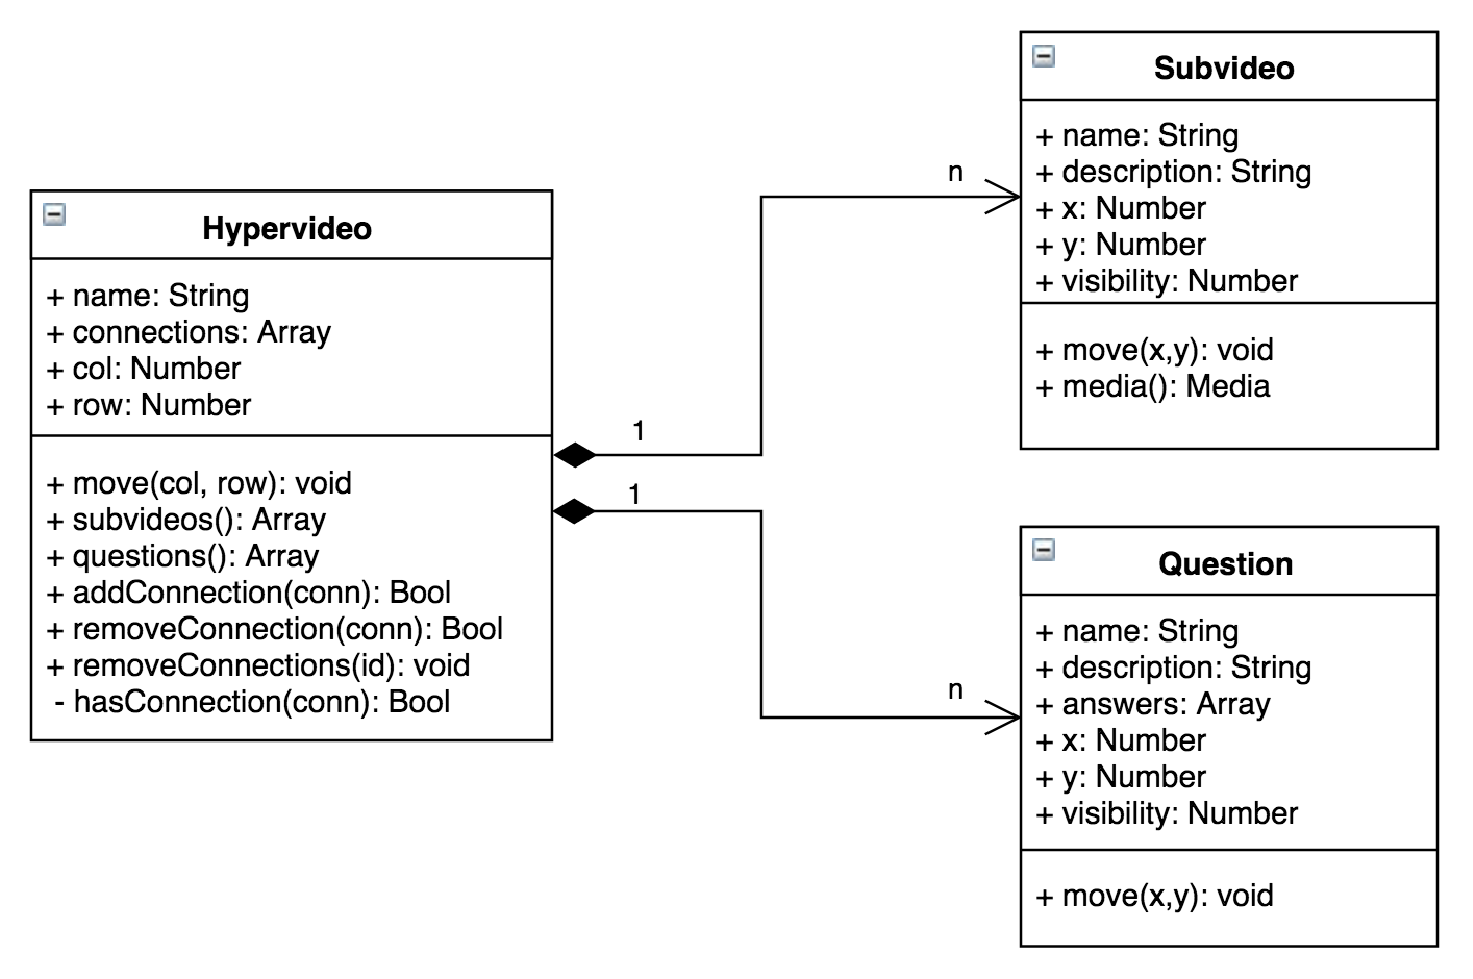
\includegraphics[width=.6\linewidth]{figuras/video.eps}
  	\caption{Diagrama do vídeo interativo proposto}
  	\label{fig:video}
\end{figure}

Primeiramente, foi modelado um vídeo interativo que pudesse ser utilizado na construção de um curso. Levando em consideração os princípios do design multimídia, os vídeos interativos possuem pouco espaço para textos escritos na tela; são formados por subvídeos interligados segundo definido pelo professor autor; possuem questões a serem respondidas ao longo da apresentação do vídeo e devem ser adaptativos segundo os diferentes perfis de usuário. Além disso, um vídeo interativo deve possuir as informações necessárias para que ocorra a quantização da rede, ou seja, para cada usuário que o acesse, deve existir uma avaliação e uma confiabilidade atribuidos a ele, bem como uma posição em um plano bidimensional referente ao mapa conceitual do curso ao qual o vídeo interativo pertence. 

\begin{figure}[h!]
	\centering
  	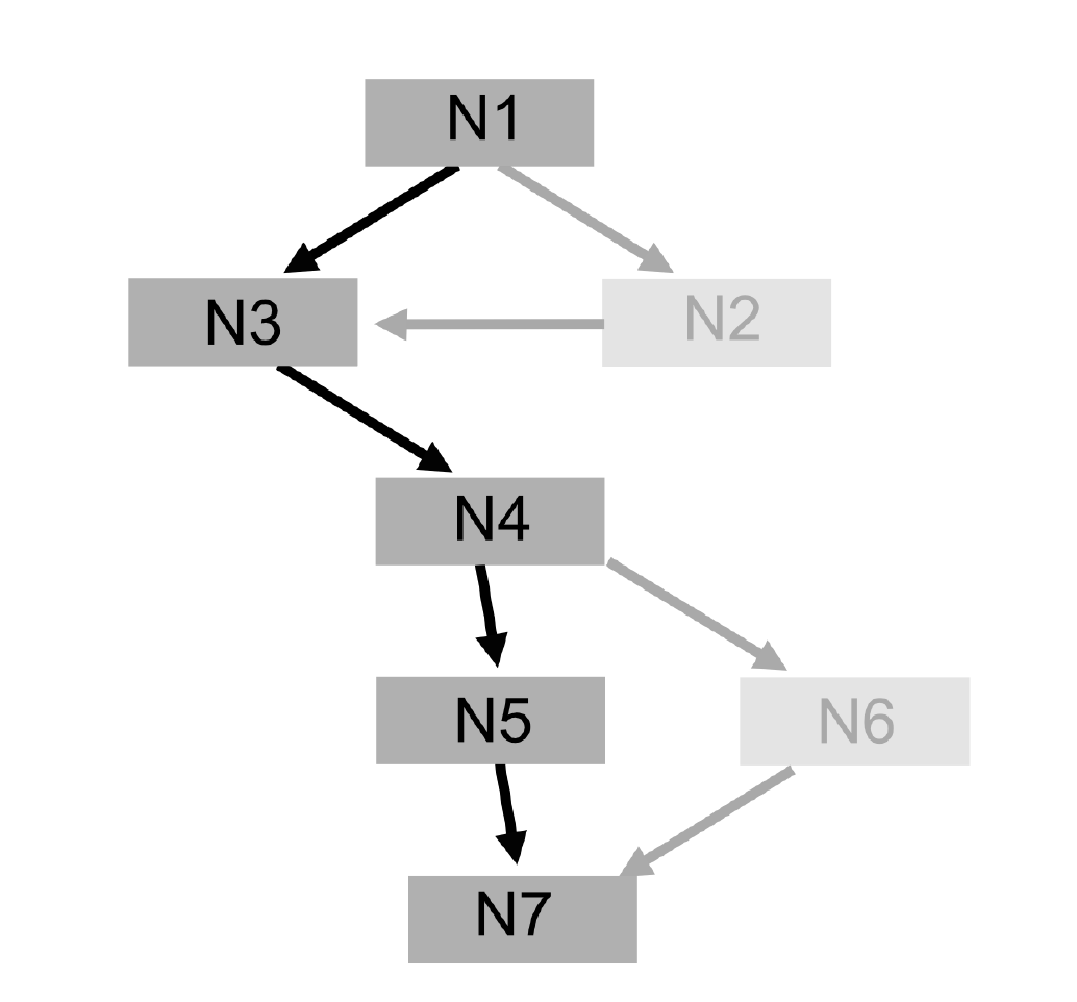
\includegraphics[width=.3\linewidth]{figuras/estrutura.eps}
  	\caption{Adaptação do hypervideo por meio da ocultação dos nodos N2 e N6}
  	\label{fig:estrutura}
\end{figure}

Cada subvídeo possui informações básicas sobre a mídia de vídeo que será apresentada por ele, como título e uma breve descrição do conteúdo. Além disso, possuem um nível de visibilidade para serem apresentados apenas ao perfil específico para o qual foi projetado, garantindo assim a capacidade de adaptação a nível de conteúdo. A fig. \ref{fig:video} apresenta um diagrama do vídeo interativo que no sistema é denominado Hypervideo.

Por meio da figura \ref{fig:video}, é possível perceber que existe uma lista de conexões para cada Hypervideo, essa lista representa o conjunto de arestas do grafo que tem como vértices os subvídeos e questões pertencentes a o vídeo interativo. Como visto no capítulo anterior, as teorias behavioristas apresentam o conteúdo de forma sequencial e linear, já as linhas cognitivistas compreendem estruturas de decisão e caminhos distintos para cada aprendiz. A figura \ref{fig:estrutura} mostra como essa estrutura de grafo pode se adaptar para adequar-se a ambas as formas de apresentação.

\begin{figure}[h!]
	\centering
  	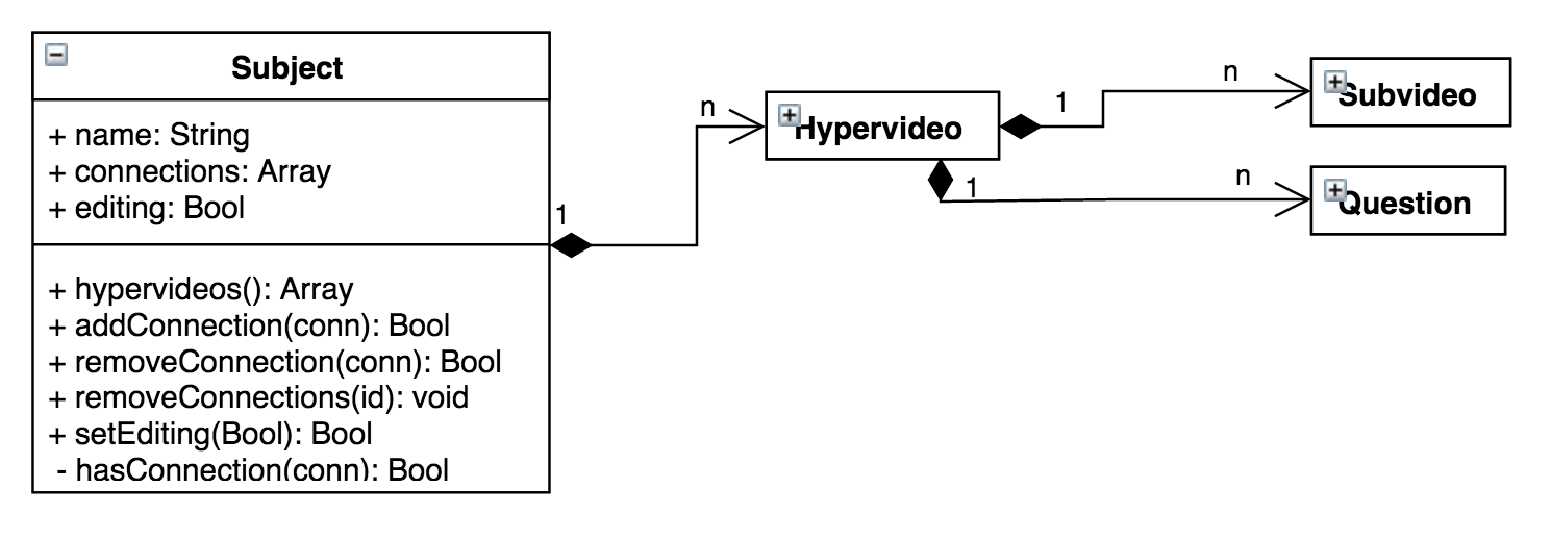
\includegraphics[width=.7\linewidth]{figuras/curso.eps}
  	\caption{Diagrama da estrutura do curso proposto}
  	\label{fig:curso}
\end{figure}

Para que fosse possível desenvolver uma adaptação da navegação que utilizasse a QRN, foi necessário modelar também a estrutura do curso que comportasse os hypervídeos e as informaçõs necessárias para os cálculos. Dessa forma, é proposto que um curso possua também, uma estrutura de grafo que tenha como vértices os seus Hypervideos, e que as conexões criadas pelo professor representem as ligações conceituais entre os tópicos apresentados em cada hypervídeo. A figura \ref{fig:curso} apresenta o modelo relativo ao curso que foi denominado \textit{Subject}.

A próxima modelagem feita foi referente aos dados do usuário: cursos que assiste, cursos construídos por ele, percentual de conclusão de um curso, questões respondidas, hypervideos assistidos, etc. Todas essas informações requereram modelos que vinculassem cada elemento de um curso ao usuário para que se pudesse calcular os coeficientes de quantização para os nodos da rede. A figura \ref{fig:userdata} mostra o modelo de domínio completo do \textit{software}.

\begin{figure}[h!]
	\centering
  	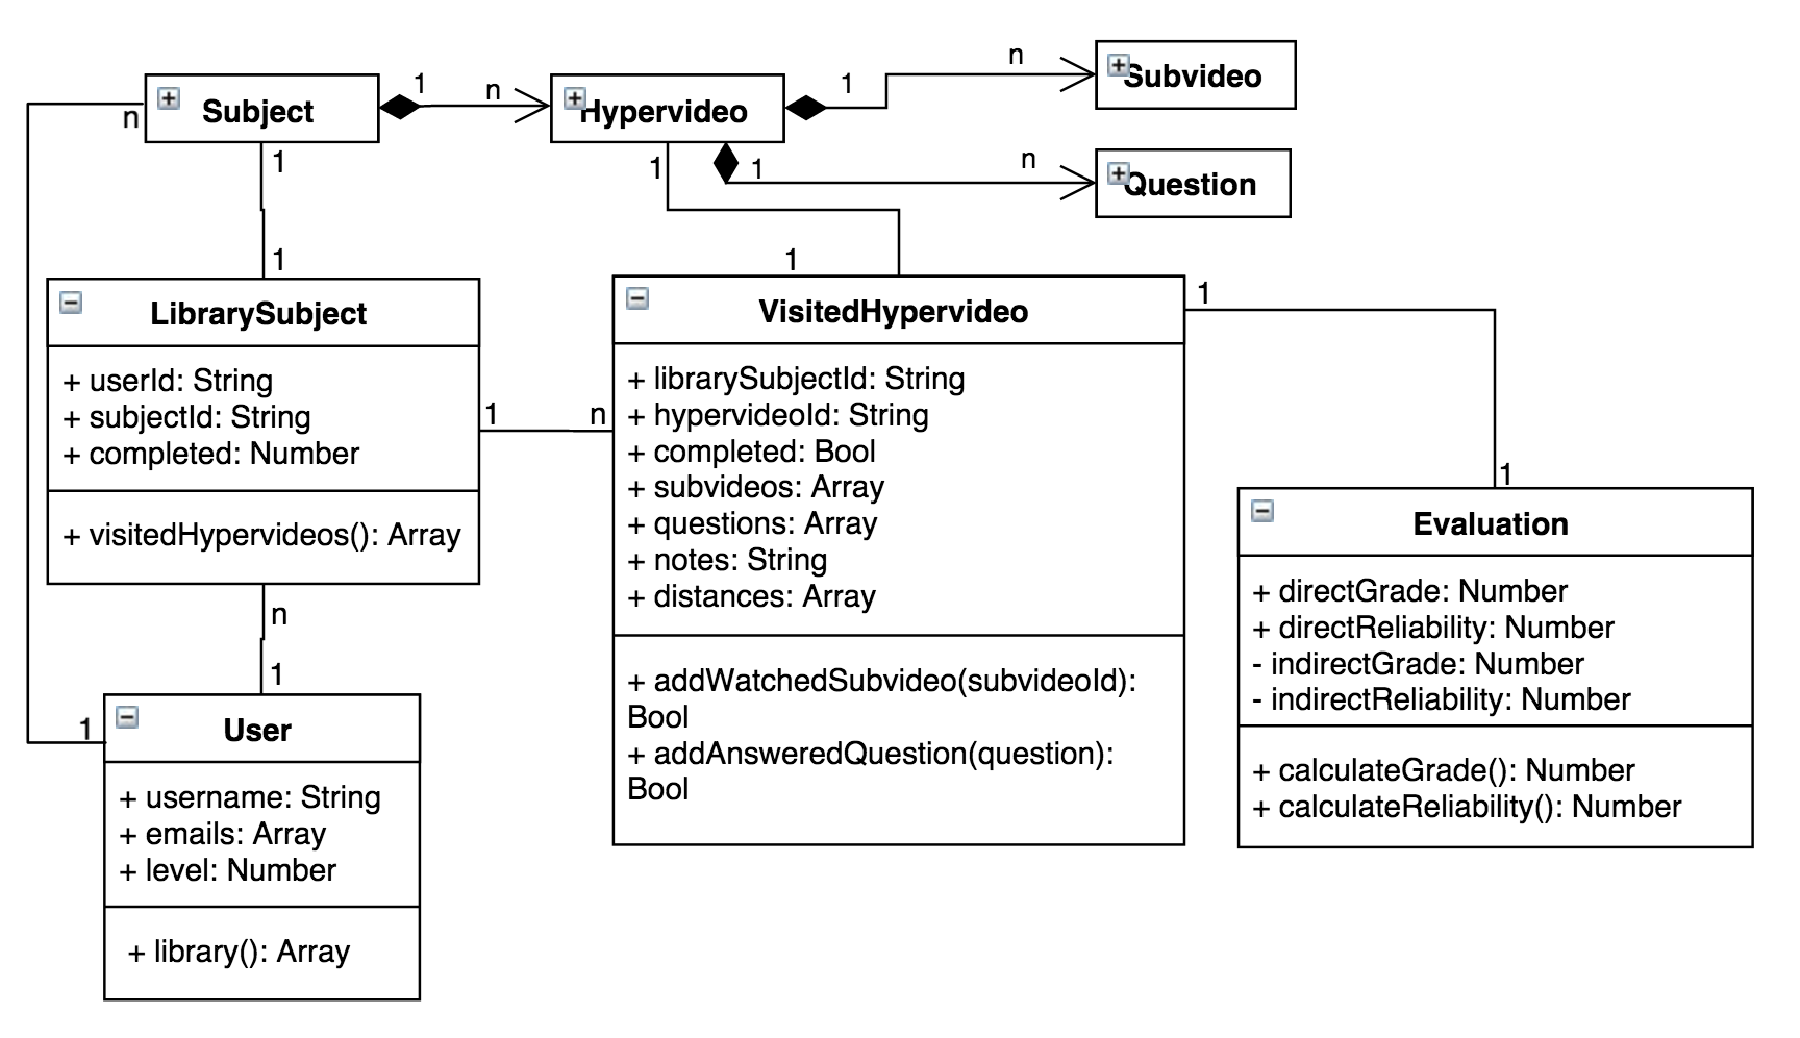
\includegraphics[width=.8\linewidth]{figuras/userdata.eps}
  	\caption{Diagrama sobre informações referentes a relação usuário \(\times\) curso}
  	\label{fig:userdata}
\end{figure}

Como a quantização da rede é definida de forma diferente para cada usuário, os cálculos da avaliação e confiabilidade diretas e indiretas devem estar vinculados ao objeto que interconecta o usuário ao nodo da rede que se pretende calcular a quantização. Dessa forma, para cada usuário que se cadastre na rede e assista a algum curso, uma quantização diferente será gerada segundo a sua interação com o sistema.

\section{Suporte Tecnológico}

Sobre o ponto de vista arquitetural, foram elicitadas ferramentas que proporcionassem maiores facilidades para o desenvolvimento do sistema. Nesse sentido, foram selecionados três \textit{frameworks} que possibilitam o desenvolvimento de aplicações \textit{web} com certo nível de abstração arquitetural, que são mantidos segundo licenças de software livre e que possuem comunidades ativas. Sendo estes: Grails \cite{grails2015}, Ruby on Rails \cite{rubyrails2015}, e Meteor \cite{meteor2015}. 
\\
\\

Para avaliar as ferramentas selecionadas, foi construído um cenário de prova de conceito, com a finalidade de verificar o esforço necessário para se implementar um pequeno software de manutensão de usuários nas três ferramentas. Os resultados coletados são descritos na tabela \ref{tab:tempo} abaixo:

\begin{table}[h!]
	\centering
	\begin{tabular}{| c | c |}
		\hline
		\textit{Framework} & Tempo \\
		\hline
		Meteor & 37 min \\
		\hline
		Rails & 44 min \\
		\hline
		Grails & 74 min \\
		\hline
	\end{tabular}
	\caption{Tempo para implementação da funcionalidade}
	\label{tab:tempo}
\end{table}

Os \textit{frameworks} Grails e Ruby on Rails possuem estilos arquiteturais bastante semelhantes, já que ambos são orientados a convensão, e possuem ferramentas de terminal interativo para criação e adição de elementos do sistema, como modelos, visões, controladoras e \textit{plugins}. Entretanto, o tempo para se desenvolver a funcionalidade com Ruby on Rails foi menor devido aos menores problemas com a configuração do ambiente de desenvolvimento e dependências do \textit{framework}.

Uma das vantagens da utilização do Ruby on Rails para o desenvolvimento é que a comunidade é bastante ativa e existe documentação abrangente sobre vários dos plugins que são disponibilizados para a plataforma. Porém, a configuração de uma ferramenta para renderização no cliente não é trivial e as complicações com a construção de APIs para comunicação remota e com a utilização de plugins JSON para recuperar dados do servidor impossibilitaram a construção da funcionalidade com este recurso.

Para a plataforma Grails, os mesmos problemas foram encontrados para a construção de uma aplicação com renderização no cliente, além dos problemas com configuração de ambiente e tempo de desenvolvimento da funcionalidade. A vantagem em se optar por utilizar uma ferramenta Java é a facilidade em se adicionar recursos multiagentes, já que existem ferramentas consolidadas como o JADE \cite{jade2015} que são mantidos nessa linguagem. Como o foco deste trabalho não abrange o desenvolvimento de agentes, este \textit{framework} foi descartado.

O processo de instalação e utilização da plataforma Meteor foi sem dúvidas o mais simples, todas as dependências do sistema são mantidas por meio do gerenciador de pacotes do Node.js \cite{nodejs2015} e foram instaladas sem nenhum empecilho. Apenas o processo simplificado de instalação não garante ao Meteor sua escolha como plataforma de desenvolvimento, além disso, o tempo para se implementar a funcionalidade proposta foi o menor dentre as plataformas, apresentou maior facilidade na construção de aplicações com renderização no cliente, possui comunidade ativa e releases frequentes de novas versões e mantém também mecanismos de teste e depuração para as aplicações Meteor, em sua maioria sob licenças de sotware livre compatíveis com a licença GPL v3 adotada neste projeto.

A opção por uma ferramenta que facilite a renderização no cliente é uma necessidade da proposta para construção do curso, já que para criar um grafo de hypervideos em um curso, ou um grafo de subvideos e questões dentro de um hypervideo, tem-se a necessidade de se construir uma biblioteca para permitir a interação com o usuário sem que, a cada interação, se gere uma nova renderização da página proveniente do servidor, e que evite perda de dados caso ocorra perda de conexão com a \textit{internet}. Arquiteturas construídas com Ruby on Rails ou Grails não oferecem suporte esse tipo de interação, exigindo bibliotecas externas à plataforma e o conhecimento em linguagens de programação diferentes das utilizadas nativamente no \textit{framework}, como \textit{JavaScript} ou \textit{CoffeScript}.

Com esta análise, optou-se pela plataforma \textit{Meteor} devido às facilidades encontradas e também pela necessidade de domínio em apenas uma linguagem: o \textit{JavaScript}. A lista completa de pacotes e ferramentas utilizadas se encontra no Apêndice A. 

\section{Arquitetura do Sistema}

